\documentclass[fleqn,twoside,twocolumn,nofootinbib,showkeys]{revtex4} % Specifies the document class %,unsortedaddress
\usepackage[sec,doi]{ujp_UTF8} % \usepackage[cyr]{ujp_UTF8} for cyrillic

\usepackage{physics}
%\usepackage{caption}

\usepackage{hyperref} % for hyperlinks in references
\usepackage[nameinlink]{cleveref}

\begin{document}
\title[Critical temperature determination for fluids]%колонтитул
{CRITICAL TEMPERATURE DETERMINATION FOR FLUIDS. AN ANALYTICAL APPROACH BASED ON COLLECTIVE VARIABLES METHOD}%
\author{I.R.~Yukhnovkii}%1 автор
\author{R.V.~Romanik}
\affiliation{Institute for Condensed Matter Physics,\\ Nat. Acad. of Sci. of Ukraine}%институт
\address{1, Svientsitskii Str., Lviv 79011, Ukraine}%адрес
\email{romanik@icmp.lviv.ua}%e-mail


\udk{539} \pacs{71.20.Nr, 72.20.Pa} \razd{\secvii}

\autorcol{R.V.~Romanik, I.R.~Yukhnovskii}

\cit{Romanik~R.V., Yukhnovskii~I.R. Critical temperature determination for fluids. An analytical approach based on collective variables method}{\selectlanguage{ukrainian} Романік~Р.В., Юхновський~І.Р. Визначення критичної температури флюїдів. Аналітичний підхід на основі методу колективних змінних}

\setcounter{page}{53}
%\setcounter{jnumber}{5}

\begin{abstract}
An explicit equation for the liquid-vapour critical temperature of simple fluids is derived within an analytical approach -- the method of collective variables with a reference system.
This equation is applied to calculate the critical temperature values for several hard-core van der Waals fluids. The study also examines how the critical temperature depends on parameters of interaction. Specifically, it is observed that as the range of attractive interaction decreases, the critical temperature decreases as well.
\end{abstract}

\keywords{Simple fluids, Collective variables, Critical temperature.}

\maketitle

\section{Introduction}

Nowadays, computer simulations seem to be the most common tool to study the equilibrium properties of simple fluids. Still, analytical theories enabling one to calculate the thermodynamic properties of many-particle interacting systems is of invaluable importance, as they may give rise to physical understanding that otherwise would be missed. One of such theories is built around the collective variables method~\cite{Yukh1980book} with a reference system~\cite{Yukh1990}. A general overview of this approach and results obtained in its framework for liquid-gas systems near the critical point can be found in~\cite{Yukh2015En}. In this paper we focus on the details of of determining the critical temperature and how the parameters of the attractive interaction affect this temperature. 

The structure of this paper is as follows. We start with presenting the explicit functional of the grand partition function, with all coefficients explicitly defined. Then we proceed with the ``layer-by-layer'' integration of that functional to obtain a sequence of effective block Hamiltonians each characterized by its coefficients. After the result of integration over $n$ layers is written down in a generic form, we pass to the analysis of the recurrence relations between the effective Hamiltonian coefficients. As a result, we find the fixed point solution, write the recurrence relations in the linear approximation around the fixed point, and find the condition resulting into the equation for the critical temperature. In Section~\ref{sec:results} we calculate the critical temperature using the found expression for different hard-core van der Waals fluids and compare the obtained values with known results for the considered models.



\section{\label{sec:init-gpf} Grand partition function in the representation of collective variables}
The grand partition function (GPF) of a simple many-particle interacting system can be represented as~\cite{Yukh1990,YukhJSP1995,RomaJPS2024}
\begin{equation}
	\label{Xi_as_prod}
	\Xi = \Xi_0\Xi_G\Xi_L.
\end{equation}
Here $\Xi_0$ is the GPF of a reference system (RS), which is assumed to be known. $\Xi_G$ is a short-wave contribution to the GPF with wave-vectors $\abs{\vb{k}}>B_0$, $B_0$ being the cut-off parameter.
The quantity $\Xi_L$ denotes long-wave contributions to the GPF and is the object of our investigation in this paper. In our previous paper~\cite{RomaJPS2024} we provided very detailed derivation of the expression for $\Xi_L$ (see~\cite{Roma2023Preprint} for even more details) and presented it as follows:
\begin{equation}
	\label{Xi_L}
	\Xi_L = j_0Q(\tilde{\mathfrak{M}_2}, \mathfrak{M}_4)^{N_0} \exp(\tilde{\mathfrak{M}}_0) \Xi_L^{(1)},
\end{equation} 
where $j_0=\sqrt{2}^{N_0 - 1},$ $N_0$ being determined in~\eqref{def:NB} below, $Q(\tilde{\mathfrak{M}_2}, \mathfrak{M}_4)$ and $\tilde{\mathfrak{M}_0}$ are explicitly given in Appendix~\ref{sec:app-a}.

The quantity $\Xi_L^{(1)}$ in the approximation of the so-called $\rho^4$ model is given by
\begin{eqnarray}
	\label{Xi_L_1}
	\Xi_L^{(1)} &=& 
	\int \exp\left(
	\mu^* \rho_0 - \frac{1}{2} \sum_{\substack{\vb k \\ k \leq B_0}} d_2(k) \rho_{\vb k} \rho_{-\vb k} 
	\right.\\
	& - & \left. \frac{a_4}{4! N_0} \sum_{\substack{\vb k_1, \dotsc, \vb k_4 \\ k_i \leq B_0}} \rho_{\vb k_1} \dotsc \rho_{\vb k_4} \delta_{\vb{k}_1 + \dotsc + \vb{k}_4} \right) ({\rm d} \rho)^{N_0}
	\nonumber.
\end{eqnarray}
Here $d_2(k) = a_2 + \frac{\beta\hat{\Phi}_{\vb k}}{V}$, $\beta$ being the inverse temperature, $V$ the volume, $\hat{\Phi}_{\vb k}$ the Fourier component of the long-range part of the interaction potential.
Quantities $\mu^*$, $a_2$ and $a_4$ are functions of the RS particle density $\rho$, temperature $T$, and microscopic parameters of interaction potential. They are explicitly presented in Appendix~\ref{sec:app-a}. The quantity $\mu^*$ also linearly depends on the chemical potential $\mu$.

The wave vector $\vb k$ takes on $N_0$ values in a sphere of radius $B_0$, so that
\begin{equation}
	\label{def:NB}
	N_0 = \frac{B_0^3}{6\pi^2}V.
\end{equation}
Thus the number of variables to be integrated over is equal to $N_0$
\begin{equation*}
	(d\rho)^{N_0} = {\rm d}\rho_0 \prod_{\substack{\vb k \\ k\le B_0}}' {\rm d}\rho_{\vb k}^c {\rm d}\omega_{\vb k}^s
\end{equation*}
where $\rho_{\vb k}^c$ and $\rho_{\vb k}^s$ are the real and imaginary parts of the collective variable $\rho_{\vb k} = \rho_{\vb k}^c - {\rm i} \rho_{\vb k}^s$, respectively\footnote{Traditionally, the collective variables are denoted by $\rho_{\vb k}$, and the element of integration over CVs is denoted by $({\rm d} \rho)$, while the particle density is denoted by $\rho$. We hope that it is clear from the context when $\rho$ is understood as the number density, and when it is related to CVs}. The `prime' sign over the product means that the wave-vector takes on values only form the upper semi-sphere, i.e. $k_z > 0$ and $\abs{\vb k} \neq 0$.

The following simplification is used for the Kronecker symbol in~\eqref{Xi_L_1}
\begin{equation*}
	\delta_{\vb k} = \frac{1}{V} \int \rm{e}^{-{\rm i} \vb k \vb r} \rm{d} \vb r = \frac{1}{N_0}\sum_{\vb l_0} {\rm e}^{-{\rm i} \vb k \vb l_0}.
\end{equation*}
The summation over $\vb l_0$ implies that $\vb l_0$ takes on $N_0$ values in real space corresponding to the $N_0$ values of wave vector $\vb k$ in a sphere of radius $B_0$ in the reciprocal space. This is called a spherical approximation for the first Brillouin zone. It is assumed that a proper correspondence can be established between a spherical Brillouin zone and a structure in real space by analogy to how simple cubic lattice corresponds to its Brillouin zone in the Ising-model problem~\cite{Yukh2001book}. 

In what follows we also will understand that $\vb l \in \Lambda_0$ corresponds to vectors $\vb k$ such that $k \leq B_0$, $\vb l \in \Lambda_1$ to $k \leq B_1$, and in general $\vb l \in \Lambda_n$ to $k \leq B_n$. Here $B_n = B_0/s^n$ and $s$ is the renormalization parameter to be introduced later.

The expression~\eqref{Xi_L_1} formally coincides with the expression for the partition function functional of the 3-dimentional Ising-like model in an external field~\cite{Mpk2012book,MpkRoma2012}. 

A necessary condition for this functional to give rise to a critical-point solution is $\mu^* = 0$, which leads to a line of critical temperature dependence on the chemical potential $\mu$ (at some value of the RS particle density $\rho_c$)~\cite{RomaJPS2024}.

We are going to integrate~\eqref{Xi_L_1} following the method developed for calculation of the partition function of the 3-dimentional Ising-like models \cite{Yukh1989riv,Yukh2001book,MpkCMP2005}. The main idea is to divide the interval $[0, B_0]$ into sub-intervals $(B_1, B_0]$, $(B_2, B_1]$, $(B_3, B_2]$ and so on, where $B_1 = B_0/s$, $B_2 = B_1/s = B_2/s^2$, or in general $B_n = B_0/s^n$, $s$ being the renormalization group parameter, $s > 1.$ Variables $\rho_{\vb k}$ with $B_1 < k \leq B_0$ are said to belong to the first layer, $\rho_{\vb k}$ with $B_2 < k \leq B_1$ to the second one, and continuing in the same manner, $\rho_{\vb k}$ with $B_n < k \leq B_{n-1}$ to the $n$-th layer.
The integration is performed iteratively, starting with integration over the collective variables of the first layer, then over the second one and so on.
The number of variables to be left after the integration over the first layer is $N_1 = N_0 / s^3 = (B_0^3 V)/(2\pi^2 s^3)$. Thus the number of variables integrated out in the first iteration is $N_0 - N_1 = N_0(1-s^{-3})$.

To factorize the integrals the Fourier transform $\hat{\Phi}_{\vb k}$ of the long-range part of interaction potential is replaced with its average value over each interval:
\begin{eqnarray*}
	\hat{\Phi}_{\vb k} & \rightarrow & \hat{\Phi}_{B_1, B_0}, \quad B_1 < k \leq B_0;
	\\
	& & \hat{\Phi}_{B_2, B_1}, \quad B_2 < k \leq B_1;
	\\
	& & ...
	\\
	& & \hat{\Phi}_{B_n, B_{n-1}}, \quad B_n < k \leq B_{n-1}.
\end{eqnarray*}
The particulars of this averaging are not so important to outline the method of layer-by-layer integration. Thus we will return to them later when we present some numerical and graphical results.
Note the we postpone the specifying of the interaction potential details to a later stage of the paper. For now, we just restrict it to a form that it can be (quite freerely) separated into short-range repulsive and long-range attractive counterparts.
The properties of the short-range one are assumed to be known. One of the required properties for the long-range part is that it possesses a Fourier transform, and the long-wave limit ($\abs{\vb k} = 0$) of it takes on a negative value.

\subsection{Integration over the first layer}
Now let us explicitly integrate over the variables of the first layer. During the course of integration we closely follow steps described in~\cite{MpkCMP2005}.

The second term in the exponent of~\eqref{Xi_L_1} is rewritten as
\begin{eqnarray*}
	\sum_{\substack{\vb k, k \leq B_0}} d_2(k) \rho_{\vb k} \rho_{-\vb k} 
	& = &  
	\sum_{\substack{\vb k, k \leq B_1}} d_2(k) \rho_{\vb k} \rho_{-\vb k}
	\\
	& + &
	\sum_{\substack{\vb k, B_1 < k \leq B_0}} d_2(B_1, B_0) \rho_{\vb k} \rho_{-\vb k}
\end{eqnarray*}
where $d_2(B_1, B_0) = a_2 + \beta\hat{\Phi}_{B_1, B_0}/V$.
The expression for $\Xi_L^{(1)}$ is now recast
\begin{eqnarray*}
	\Xi_L^{(1)} &=& 
	\int \exp\left(
	\mu^* \rho_0 - \frac{1}{2} \sum_{\substack{\vb k \\ k \leq B_1}} d_2(k) \rho_{\vb k} \rho_{-\vb k}
	\right.
	\\
	& - & 
	\left.
	\frac{d_2(B_1, B_0)}{2} \sum_{\substack{\vb k \\ B_1 < k \leq B_0}} \rho_{\vb k} \rho_{-\vb k}  
	\right.
	\\
	& - & \left. \frac{a_4}{4! N_0} \sum_{\substack{\vb k_1, \dotsc, \vb k_4 \\ k_i \leq B_0}} \rho_{\vb k_1} \dotsc \rho_{\vb k_4} \delta_{\vb{k}_1 + \dotsc + \vb{k}_4} \right)
	\\ 
	& \times & ({\rm d} \rho)^{N_1} ({\rm d} \rho)^{N_0 - N_1}.
\end{eqnarray*}
To distinguish the variables to be integrated over in the first iteration, let us denote them by $\eta_{\vb k}$, i.e. $\rho_{\vb k} \rightarrow \eta_{\vb k}$ for $B_1 < k \leq B_0$. Let us also extend the number of variables $\eta_{\vb k}$ with the help of $\delta-$functions:
\begin{eqnarray*}
	\prod_{\vb{k}, 0\leq k \leq B_1}\delta(\eta_{\vb k}-\rho_{\vb k})
	& = &  \int ({\rm d}\nu)^{N_1} \\
	&\times& \exp (2\pi{\rm i}\sum_{k\leq B_1}\nu_{\vb k}(\eta_{\vb k}-\rho_{\vb k}))
\end{eqnarray*}
so that $\Xi_L^{(1)}$ is rewritten as 
\begin{eqnarray*}
	\Xi_L^{(1)} &=& 
	\int ({\rm d} \rho)^{N_1} \exp 
	\Bigl(
		\mu^* \rho_0 
		%\right.
	\\
	& - & 
	\left.\frac{1}{2} \sum_{\substack{\vb k \\ k \leq B_1}} (d_2(k) - d_2(B_1, B_0) ) \rho_{\vb k} \rho_{-\vb k}
	\right)
	\\
	&\times&  \int ({\rm d}\nu)^{N_1} \exp \left(-2\pi{\rm i}\sum_{\vb k, k \leq B_1} \nu_{\vb k}\rho_{\vb k}\right)
	I(\nu_{\vb k}).
\end{eqnarray*}
Here the notation $I(\nu_{\vb k})$ stands for the integral over $\eta_{\vb k}$
\begin{eqnarray*}
	I(\nu_{\vb k}) & = & \int ({\rm d} \eta)^{N_0} \exp
	\left( 2\pi{\rm i} \sum_{\vb k, k \leq B_0} \bar{\nu}_{\vb k} \eta_{\vb k} 
	\right.
	\\
	&-& \left. \frac{d_2(B_1, B_0)}{2} \sum_{\vb k, k \leq B_0} \eta_{\vb k} \eta_{-\vb k}
	\right.
	\\
	&& - \left. \frac{a_4}{4! N_0} \sum_{\substack{\vb k_1, \dotsc, \vb k_4 \\ k_i \leq B_0}} \eta_{\vb k_1} \dotsc \eta_{\vb k_4} \delta_{\vb{k}_1 + \dotsc + \vb{k}_4} \right)
\end{eqnarray*}
where the quantity $\bar{\nu}_{\vb k}$ is introduced as
\begin{equation*}
	\bar{\nu}_{\vb k} = \left\{
	\begin{array}{ll}
		\nu_{\vb k}, \quad k \leq B_1, \\
		0, \quad B_1 < k \leq B_0
	\end{array}
	\right.
\end{equation*}
by analogy with the method described in~\cite{MpkCMP2005}.

Now this integral can be factorized in the so-called site variables
\begin{eqnarray*}
	\tilde{\eta}_{\vb l} & = & \frac{1}{\sqrt{N_0}}\sum_{\vb k, k \leq B_0}\eta_{\vb k}{\rm e}^{{\rm i}{\vb k}{\vb l}},
	\\
	\tilde{\bar{\nu}}_{\vb l} & = &\frac{1}{\sqrt{N_0}}\sum_{\vb k, k \leq B_0}\bar{\nu}_{\vb k}{\rm e}^{-{\rm i}{\vb k}{\vb l}}.
\end{eqnarray*}
For some useful relations for site variables, see Appendix~\ref{sec:app-b}.
Now the integral takes on the form
\begin{eqnarray*}
	I(\nu_{\vb k}) & = & j_0^{-1} \prod_{\vb l \in \Lambda_0} \int_{-\infty}^{\infty} {\rm d} \tilde{\eta_{\vb l}}
	\exp\Bigl( 2\pi{\rm i} \tilde{\bar{\nu}}_{\vb l} \tilde{\eta_{\vb l}} 
	%\right.
	\\
	&& 
	\left. -\frac{d_2(B_1, B_0)}{2} \tilde{\eta_{\vb l}}^2 - \frac{a_4}{4!}\tilde{\eta_{\vb l}}^4 \right)
	\\
	& = & j_0^{-1} [Q_{f_0}]^{N_0} \prod_{\vb l \in \Lambda_0} \exp(-\sum_{n \geq 1} \frac{S_{2n}}{(2n)!} \tilde{\bar{\nu}}_{\vb l}^{2n}).
\end{eqnarray*}
Restricting the resulting exponent to the $4$-th power in $\tilde{\bar{\nu}}_{\vb l}$ one gets
\begin{eqnarray*}
	I(\nu_{\vb k}) & = & j_0^{-1} [Q_{f_0}]^{N_0} \prod_{\vb l \in \Lambda_0}
	\exp(-\frac{S_2}{2!}\tilde{\bar{\nu}}_{\vb l}^2 - \frac{S_4}{4!}\tilde{\bar{\nu}}_{\vb l}^4 ).
\end{eqnarray*}
In terms of $\nu_{\vb k}$ the result for $I(\nu_{\vb k})$ is expressed as follows:
\begin{eqnarray*}
	I(\nu_{\vb k}) & = & j_0^{-1} [Q_{f_0}]^{N_0} 
	\exp \left(- \frac{S_2}{2!} \sum_{\vb k, k \leq B_1} \nu_{\vb k} \nu_{-\vb k}
	\right.
	\\
	& - & \left.
	 \frac{S_4}{4! N_0} \sum_{\substack{\vb k_1, \dotsc, \vb k_4 \\ k_i \leq B_1}} \nu_{\vb k_1} \dotsc \nu_{\vb k_4} \delta_{\vb{k}_1 + \dotsc + \vb{k}_4}
	 \right)
	 .
\end{eqnarray*}
In the above formulae, the following quantities were introduced:
\begin{equation*}
	Q_{f_0} = \sqrt{2\pi}\left(\frac{3}{a_4}\right)^{1/4} {\rm e}^{x^2/4} U(0,x);
\end{equation*}
\begin{equation*}
	S_2 = (2\pi)^2 \left(\frac{3}{a_4}\right)^{1/2} U(x); \quad S_4 = (2\pi)^4 \frac{3}{a_4}\varphi(x);
\end{equation*}
\begin{equation*}
	x = d_2(B_1, B_0) \left(\frac{3}{a_4}\right)^{1/2}.
\end{equation*}

The next step is to integrate over $\nu_{\vb k}$ the following integral
\begin{eqnarray*}
	I_2(\rho_{\vb k}) & = & \int ({\rm d} \nu)^{N_1} 
	\exp 
	\left(-2\pi{\rm i} \sum_{\vb k, k \leq B_1} \nu_{\vb k}\rho_{\vb k}
	\right.
	\\
	&-&
	\left.
	 \frac{S_2}{2!} \sum_{\vb k, k \leq B_1} \nu_{\vb k}\nu_{-\vb k}
	\right.
	\\
	& - &
	\left. 
		\frac{S_4 s^{-3}}{4! N_1} \sum_{\substack{\vb k_1, \dotsc, \vb k_4 \\ k_i \leq B_1}} \nu_{\vb k_1} \dotsc \nu_{\vb k_4} \delta_{\vb{k}_1 + \dotsc + \vb{k}_4}
	\right)
	\\
	& = &
	j_1 \prod_{\vb l \in \Lambda_1} \int {\rm d} \tilde{\nu}_{\vb l} 
	\exp(-2\pi {\rm i} \tilde{\nu}_{\vb l} \tilde{\rho}_{\vb l})
	\\
	&& \times \exp(- \frac{S_2}{2!}\tilde{\nu}_{\vb l}^2
	- \frac{S_4}{4! s^3} \tilde{\nu}_{\vb l}^4  )
\end{eqnarray*}
where $j_1 = \sqrt{2}^{N_1 - 1}$, and this time
\begin{eqnarray*}
	\tilde{\rho}_{\vb l} & = &  \frac{1}{\sqrt{N_1}}\sum_{\vb k, k \leq B_1}\rho_{\vb k}{\rm e}^{{\rm i}{\vb k}{\vb l}}
	,
	\\
	\tilde{\nu}_{\vb l} & = & \frac{1}{\sqrt{N_1}}\sum_{\vb k, k \leq B_1}\nu_{\vb k}{\rm e}^{-{\rm i}{\vb k}{\vb l}}.
\end{eqnarray*}
The result of integration is
\begin{equation*}
	I_2(\rho_{\vb k}) = j_1 [Q_{\varphi_0}]^{N_1} \prod_{\vb l \in \Lambda_1} 
	\exp(- \sum_{n \geq 1} \frac{R_{2n}}{(2n)!} \tilde{\rho}_{\vb l}^{2n} ).
\end{equation*}
In the "$\rho^4$" approximation this takes the form
\begin{eqnarray*}
	I_2(\rho_{\vb k}) & = & j_1 [Q_{\varphi_0}]^{N_1} \prod_{\vb l \in \Lambda_1}
	\exp( - \frac{R_2}{2!} \tilde{\rho}_{\vb l}^2 - \frac{R_4}{4!} \tilde{\rho}_{\vb l}^4)
	\\
	& = & j_1 [Q_{\varphi_0}]^{N_1} 
	\exp\left( -\frac{R_2}{2!} \sum_{\vb k, k \leq B_1} \rho_{\vb k} \rho_{-\vb k} 
	\right.
	\\
	&& - \left. \frac{R_4}{4!N_1} 
	\sum_{\substack{\vb k_1, \dotsc, \vb k_4 \\ k_i \leq B_1}} \rho_{\vb k_1} \dotsc \rho_{\vb k_4} \delta_{\vb{k}_1 + \dotsc + \vb{k}_4}\right).
\end{eqnarray*}
Here
\begin{equation*}
	Q_{\varphi_0} = (2\pi)^{-1/2} s^{3/4} \left(\frac{a_4}{\varphi(x)}\right)^{1/4} {\rm e}^{y^2/4} U(0,y);
\end{equation*}
\begin{equation*}
	R_2 = s^{3/2} \left(\frac{a_4}{\varphi(x)}\right)^{1/2} U(y); \quad R_4 = s^3 a_4 \frac{\varphi(y)}{\varphi(x)};
\end{equation*}
\begin{equation*}
	y = s^{3/2} U(x) \sqrt{\frac{3}{\varphi(x)}}.
\end{equation*}
This time the approximation for the Kronecker symbol is 
\begin{equation*}
	\delta_{\vb k} \approx \frac{1}{N_1} \sum_{\vb l \in \Lambda_1} \exp(-{\rm i} \vb{k} \vb{l}).
\end{equation*}

Finally, as a result of integration over the first layer, we get for $\Xi_L^{(1)}$
\begin{eqnarray*}
	&& \Xi_L^{(1)} = j_0^{-1}j_1 [Q_{f_0}]^{N_0} [Q_{\varphi_0}]^{N_1} 
	\\
	&& \times 
	\int ({\rm d} \rho)^{N_1} \exp
	\left(
	\mu^*\rho_0 - \frac{1}{2} \sum_{\vb k, k \leq B_1} d_2^{(1)}(k) \rho_{\vb k} \rho_{-\vb k}
	\right.
	\nonumber \\
	&& -  
	\left.
	\frac{a_4^{(1)}}{4!N_1} \sum_{\substack{\vb k_1, \dotsc, \vb k_4 \\ k_i \leq B_1}}
	\rho_{\vb k_1} \dotsc \rho_{\vb k_4} \delta_{\vb{k}_1 + \dotsc + \vb{k}_4}
	\right)
	\nonumber
\end{eqnarray*}
where
\begin{equation}
	\label{RR_1_0_d}
	d_2^{(1)}(k) = a_2^{(1)} + \beta\hat{\Phi}_{\vb k} / V;
\end{equation}
\begin{eqnarray}
	\label{RR_1_0_a2}
	a_2^{(1)} & = & R_2 - \frac{\beta\hat{\Phi}_{B_1, B_0}}{V} 
	\\
	& = & s^{3/2} \left(\frac{a_4}{\varphi(x)}\right)^{1/2} U(y)
	- \frac{\beta\hat{\Phi}_{B_1, B_0}}{V};
	\nonumber
\end{eqnarray}
\begin{equation}
	\label{RR_1_0_a4}
	a_4^{(1)} = R_4 = s^3 a_4 \frac{\varphi(y)}{\varphi(x)}.
\end{equation}
These are recurrence relations between coefficients of an effective Hamiltonian before and after the integration over the first layer, establishing expressions for coefficients $a_2^{(1)}$ and $a_4^{(1)}$ via $a_2$ and $a_4$. An alternative, concise form is
\begin{eqnarray}
	\label{RR_1_0_a2_short}
	a_2^{(1)} & = & d_2(B_1, B_0) N(x) - \frac{\beta\hat{\Phi}_{B_1, B_0}}{V};
	\\
	\label{RR_1_0_a4_short}
	a_4^{(1)} & = & s^{-3} a_4 E(x).
\end{eqnarray}
Here the following quantities are introduced
\begin{equation*}
	N(x) = \frac{y U(y)}{x U(x)}; \quad E(x) = s^6 \frac{\varphi(y)}{\varphi(x)}.
\end{equation*}

\subsection{Integration over the second layer}
Following the outlined procedure, one can perform the integration over the second layer, with $B_2 < k \le B_1.$ As a result of such integration, the quantity $\Xi_L^{(1)}$ takes on the following expression:
\begin{eqnarray*}
	&&\Xi_L^{(1)} = j_0^{-1}j_2 [Q_{f_0}]^{N_0} [Q_{\varphi_0}]^{N_1} [Q_{f_1}]^{N_1} [Q_{\varphi_1}]^{N_2} 
	\\
	&& \times 
	\int ({\rm d} \rho)^{N_2} \exp
	\left(
	\mu^*\rho_0 - \frac{1}{2} \sum_{\vb k, k \leq B_2} d_2^{(2)}(k) \rho_{\vb k} \rho_{-\vb k}
	\right.
	\nonumber \\
	&& - 
	\left.
	\frac{a_4^{(2)}}{4!N_2} \sum_{\substack{\vb k_1, \dotsc, \vb k_4 \\ k_i \leq B_2}}
	\rho_{\vb k_1} \dotsc \rho_{\vb k_4} \delta_{\vb{k}_1 + \dotsc + \vb{k}_4}
	\right)
	\nonumber ,
\end{eqnarray*}
where $j_2 = \sqrt{2}^{N_2 - 1},$ and
\begin{equation}
	\label{RR_2_1_d}
	d_2^{(2)}(k) = a_2^{(2)} + \beta\hat{\Phi}_{\vb k} / V;
\end{equation}
\begin{eqnarray}
	\label{RR_2_1_a2}
	a_2^{(2)} & = & R_2^{(1)} - \frac{\beta\hat{\Phi}_{B_2, B_1}}{V} 
	\\
	& = & s^{3/2} \left(\frac{a_4^{(1)}}{\varphi(x_1)}\right)^{1/2} U(y_1)
	- \frac{\beta\hat{\Phi}_{B_2, B_1}}{V};
	\nonumber
\end{eqnarray}
\begin{equation}
	\label{RR_2_1_a4}
	a_4^{(2)} = R_4^{(1)} = s^3 a_4^{(1)} \frac{\varphi(y_1)}{\varphi(x_1)}.
\end{equation}
The other quantities are
\begin{eqnarray*}
	R_2^{(1)} & = & s^{3/2} \left(\frac{a_4^{(1)}}{\varphi(x_1)}\right)^{1/2} U(y_1); 
	\\
	R_4^{(1)} & = & s^3 a_4^{(1)} \frac{\varphi(y_1)}{\varphi(x_1)};
\end{eqnarray*}
\begin{eqnarray*}
	y_1 & = & s^{3/2} U(x_1) \left(\frac{3}{\varphi(x_1)}\right)^{1/2};
	\\
	x_1 & = & d_2^{(1)}(B_2, B_1) \left(\frac{3}{a_4^{(1)}}\right)^{1/2}.
\end{eqnarray*}
\begin{eqnarray*}
	Q_{f_1} & = & \sqrt{2\pi}\left(\frac{3}{a_4^{(1)}}\right)^{1/4} {\rm e}^{x_1^2/4} U(0,x_1);
\\
	Q_{\varphi_1} & = & (2\pi)^{-1/2} s^{3/4} \left(\frac{a_4^{(1)}}{\varphi(x_1)}\right)^{1/4} {\rm e}^{y_1^2/4} U(0,y_1).
\end{eqnarray*}

The recurrence relations~\eqref{RR_2_1_d}~-~\eqref{RR_2_1_a4} link the coefficients of an effective Hamiltonian before and after the integration over the second layer, expressing coefficients $a_2^{(2)}$ and $a_4^{(2)}$ via $a_2^{(1)}$ and $a_4^{(1)}$. They are analogous to Eqs.~\eqref{RR_1_0_d}~-~\eqref{RR_1_0_a4}. Written in a concise form analogous to~Eqs.~\eqref{RR_1_0_a2_short} and~\eqref{RR_1_0_a4_short}, they are
\begin{eqnarray}
	a_2^{(2)} & = & d_2^{(1)}(B_2, B_1) N(x_1) - \frac{\beta\hat{\Phi}_{B_2, B_1}}{V};
	\\
	a_4^{(2)} & = & s^{-3} a_4^{(1)} E(x_1).
\end{eqnarray}

\subsection{General result for the layer-by-layer integration}
Having noticed the pattern while integration over the first two layers, we are now ready to generalize the result for an arbitrary number of layers.

\begin{eqnarray}
	&&\Xi_L^{(1)} = j_0^{-1}j_n Q_0 Q_1 \dotsc Q_{n-1} 
	\\
	&&\times 
	\int ({\rm d} \rho)^{N_n} \exp
	\left(
	\mu^*\rho_0 - \frac{1}{2} \sum_{\vb k, k \leq B_n} d_2^{(n)}(k) \rho_{\vb k} \rho_{-\vb k}
	\right.
	\nonumber \\
	&&- 
	\left.
	\frac{a_4^{(n)}}{4!N_n} \sum_{\substack{\vb k_1, \dotsc, \vb k_4 \\ k_i \leq B_n}}
	\rho_{\vb k_1} \dotsc \rho_{\vb k_4} \delta_{\vb{k}_1 + \dotsc + \vb{k}_4}
	\right)
	\nonumber ,
\end{eqnarray}
where $j_n = \sqrt{2}^{N_n - 1},$ and
\begin{eqnarray}
	\label{RR_n_d}
	d_2^{(n)}(k) & = & a_2^{(n)} + \beta\hat{\Phi}_{\vb k} / V;
\end{eqnarray}
\begin{eqnarray}
	\label{RR_n_a2}
	a_2^{(n)} & = & R_2^{(n-1)} - \frac{\beta\hat{\Phi}_{B_n, B_{n-1}}}{V}
	\\
	& = &  s^{3/2} \left(\frac{a_4^{(n-1)}}{\varphi(x_{n-1})}\right)^{1/2} U(y_{n-1})
	- \frac{\beta\hat{\Phi}_{B_n, B_{n-1}}}{V};
	\nonumber
\end{eqnarray}
\begin{eqnarray}
	\label{RR_n_a4}
	a_4^{(n)} & = & R_4^{(n-1)} = s^3 a_4^{(n-1)} \frac{\varphi(y_{n-1})}{\varphi(x_{n-1})}.
\end{eqnarray}
The other quantities are
\begin{eqnarray*}
	R_2^{(n)} & = & s^{3/2} \left(\frac{a_4^{(n)}}{\varphi(x_n)}\right)^{1/2} U(y_n);
\\
	R_4^{(n)} & = & s^3 a_4^{(n)} \frac{\varphi(y_n)}{\varphi(x_n)},
\end{eqnarray*}
\begin{eqnarray*}
	y_n & = & s^{3/2} U(x_n) \left(\frac{3}{\varphi(x_n)}\right)^{1/2},
\\
	x_n & = & d_2^{(n)}(B_{n+1}, B_n) \left(\frac{3}{a_4^{(n)}}\right)^{1/2}.
\end{eqnarray*}

\begin{eqnarray*}
	Q_n & = & Q_{f_n}^{N_n} Q_{\varphi_{n}}^{N_{n+1}};
\\
	Q_{f_n} & = & \sqrt{2\pi}\left(\frac{3}{a_4^{(n)}}\right)^{1/4} {\rm e}^{x_n^2/4} U(0,x_n);
\\
	Q_{\varphi_n} & = & (2\pi)^{-1/2} s^{3/4} \left(\frac{a_4^{(n)}}{\varphi(x_n)}\right)^{1/4} {\rm e}^{y_n^2/4} U(0,y_n).
\end{eqnarray*}
A concise form of the recurrence relations is as follows:
\begin{eqnarray*}
	a_2^{(n)} & = & d_2^{(n-1)}(B_n, B_{n-1}) N(x_{n-1}) - \frac{\beta\hat{\Phi}_{B_n, B_{n-1}}}{V};
	\\
	a_4^{(n)} & = & s^{-3} a_4^{(n-1)} E(x_{n-1}).
\end{eqnarray*}

\subsection{Recurrence relations}
The general recurrence relations between coefficients of effective block-structure Hamiltonians can be written in the form
\begin{eqnarray}
	a_2^{(n+1)} & = & d_2^{(n)}(B_{n+1}, B_n) N(x_n) - \frac{\beta\hat{\Phi}_{B_{n+1}, B_n}}{V};
	\\
	a_4^{(n+1)} & = & s^{-3} a_4^{(n)} E(x_{n}).
\end{eqnarray}
With the help of the following change of variables
\begin{eqnarray*}
	r_n & = & d_2^{(n)}(0)s^{2n},
	\nonumber \\
	u_n & = & a_4^{(n)}s^{4n},
	\nonumber
\end{eqnarray*}
the recurrence relations become
\begin{eqnarray}
	\label{RR_final}
	r_{n+1} & = & s^2(r_n + q) N(x_n) - s^2 q;
	\nonumber\\
	u_{n+1} & = & s u_n E(x_n).
\end{eqnarray}
Here
\begin{equation*}
	q = s^{2n} \frac{\beta \hat{\Phi}_0}{V} \left(\frac{\hat{\Phi}_{B_{n+1}, B_n}}{\hat{\Phi}_0} - 1\right) = -\frac{\beta \hat{\Phi}_0}{V} \bar{q},
\end{equation*}
where
\begin{equation*}
	\bar{q} = -s^{2n} \left(\frac{\hat{\Phi}_{B_{n+1}, B_n}}{\hat{\Phi}_0} - 1\right).
\end{equation*}
The recurrence relations~\eqref{RR_final} possess a fixed point solution in the limit of $n \to \infty$. By definition, the fixed point solution means
\begin{equation*}
	r_{n+1} = r_n = r^*; \quad u_{n+1} = u_n = u^*
\end{equation*}
and hence
\begin{eqnarray*}
	r^* & = & s^2[-q + (r^* + q)N(x^*)],
	\nonumber \\
	u^* & = & s u^* E(x^*).
\end{eqnarray*}
From the last equality it follows
\begin{equation*}
	sE(x^*) = 1.
\end{equation*}
It is practical to chose $x^* = 0$, which is equivalent to $\lim_{n \to \infty}d_2^{(n)}(0) = d_2^* = 0$ at the fixed point, and gives $s = s^* = 3.5862$. We will use this value of $s$ to obtain particular numerical and graphical results. From the first recurrence relation it follows
\begin{equation*}
	r^* = -q\frac{N(x^*) - 1}{N(x^*) - s^{-2}}.
\end{equation*}
At $x^* = 0$, $r^* = -q$ because 
$$
\lim_{x \to 0} \frac{N(x) -1}{N(x) - s^{-2}} = 1.
$$ 

Finally, from 
\begin{equation*}
	x^* = \sqrt{3} \frac{r^* + q}{\sqrt{u^*}}
\end{equation*}
one finds the following expression for $u^*$
\begin{equation*}
	u^* = \frac{3 q^2}{(x^*)^2} \left[\frac{1 - s^{-2}}{N(x^*) - s^{-2}}\right]^2.
\end{equation*}

We can write down the coordinates of the fixed point (for details on $\hat{\Phi}_0$, see Subsection~\ref{sec:parab_pot}):
\begin{equation}
	r^* = - {\frac{\beta \abs{\hat{\Phi}_0}}{V}} \bar{r}, 
	\quad 
	u^* = \left(\frac{\beta \hat{\Phi}_0}{V}\right)^2 \bar{u}
\end{equation}
where
\begin{equation*}
	\bar{r} = \frac{N(x^*) - 1}{N(x^*) - s^{-2}} \bar{q}, 
	\quad 
	\bar{u} = \frac{3}{(x^*)^2} \left(\frac{1 - s^{-2}}{N(x^*) - s^{-2}}\right)^2 \bar{q}^2.
\end{equation*}
We consider potentials with $\hat{\Phi}_0 < 0$, thus we write $\hat{\Phi}_0 = -\abs{\hat{\Phi}_0}$

Let us use the linear approximation for the recurrence relations~\eqref{RR_final}
\begin{equation}
	\label{eq:linear_rr}
	\left(
		\begin{array}{c}
			r_{n+1} - r^* \\
			u_{n+1} - u^*
		\end{array}
	\right)
	= \cal{R}
	\left(
		\begin{array}{c}
			r_{n} - r^* \\
			u_{n} - u^*
		\end{array}
	\right)
\end{equation}
The elements of the linearized renormalization group transformation matrix $\cal{R}$ are calculated by the formulas
\begin{equation*}
	R_{11} = \left(\frac{\partial r_{n+1}}{\partial r_n}\right)^* = s^2 \left[N(x^*) + x^* \left(\frac{\partial N(x)}{\partial x} \right)_{x=x^*} \right],
\end{equation*}
\begin{equation*}
	R_{12} = \left(\frac{\partial r_{n+1}}{\partial u_n}\right)^* = \frac{R_{12}^{(0)}}{\sqrt{u^*}},
\end{equation*}
\begin{equation*}
	R_{21} = \left(\frac{\partial u_{n+1}}{\partial r_n}\right)^* = R_{21}^{(0)} \sqrt{u^*},
\end{equation*}
\begin{equation*}
	R_{22} = \left(\frac{\partial u_{n+1}}{\partial u_n}\right)^* = s \left[E(x^*) - \frac{x^*}{2} \left(\frac{\partial E(x)}{\partial x}\right)_{x=x^*}\right].
\end{equation*}
Here the star refers to the fixed-point values, and
\begin{equation*}
	R_{12}^{(0)} = -\frac{s^2}{2\sqrt{3}} (x^*)^2 \left(\frac{\partial N(x)}{\partial x} \right)_{x=x^*},
\end{equation*}
\begin{equation*}
	R_{21}^{(0)} = s\sqrt{3} \left(\frac{\partial E(x)}{\partial x}\right)_{x=x^*}.
\end{equation*}
Note that the following relations were used for calculating the matrix elements:
\begin{equation*}
	\left(\frac{\partial x_n}{\partial r_n}\right)^* = \frac{\sqrt{3}}{\sqrt{u^*}}, 
	\quad
	\left(\frac{\partial x_n}{\partial u_n}\right)^* = - \frac{x^*}{2u^*}.
\end{equation*}

The eigenvalues for the matrix $\cal{R}$ are
\begin{eqnarray*}
	E_1 & = &  \frac{1}{2} \Bigl\{ (R_{11} + R_{22})
	\\
	&& + \left. \left[(R_{11} - R_{22})^2 + 4 R_{12}^{(0)}R_{21}^{(0)}\right]^{1/2}\right\},
\end{eqnarray*}
\begin{eqnarray*}
	E_2 & = & \frac{1}{2} \Bigl\{ (R_{11} + R_{22}) 
	\\
	&& - \left. \left[(R_{11} - R_{22})^2 + 4 R_{12}^{(0)}R_{21}^{(0)}\right]^{1/2}\right\}.
\end{eqnarray*}
The eigenvectors for the matrix $\cal{R}$ are
\begin{equation*}
	W_1 = W_{11} \left(
	\begin{array}{ll}
		1 
		\\ 
		R_1
	\end{array}
	\right)
	, \quad
	W_1 = W_{11} \left(
	\begin{array}{ll}
		R 
		\\ 
		1
	\end{array}
	\right)
\end{equation*}
where constants $W_{11}$ and $W_{22}$ are yet to be determined, and quantities $R$ and $R_1$ are defined as
\begin{eqnarray*}
	R & = & \frac{R_{12}}{E_2 - R_{11}} = (u^*)^{1/2}R^{(0)}, 
	\\
	R_1 & = & \frac{E_1 - R_{11}}{R_{12}} = (u^*)^{-1/2}R_1^{(0)},
\end{eqnarray*}
with
\begin{eqnarray*}
	R^{(0)} & = & \frac{R_{12}^{(0)}}{E_2 - R_{11}},
	\\
	R_1^{(0)} & = & \frac{E_1 - R_{11}}{R_{12}^{(0)}}.
\end{eqnarray*}
Thus, the solution to the linear recurrence relations~\eqref{eq:linear_rr} can be written as
\begin{equation}
	\left(
	\begin{array}{ll}
		r_n - r^*
		\\
		u_n - u^*
	\end{array}
	\right)
	= c'_1 W_1 E_1^n + c'_2 W_2 E_2^n,
\end{equation}
where $c'_1$ and $c'_2$ are some constants. We arrive at the following equatinos for $r_n$ and $u_n$:
\begin{eqnarray}
	r_n & = & r^* + c_1 E_1^n + c_2 R E_2^n,
	\nonumber \\
	u_n & = & u^* + c_1 R_1 E_1^n + c_2 E_2^n,
\end{eqnarray}
where $c_1 = W_{11} c'_1$ and $c_2 = W_{22} c'_2$ are to be determined from the initial conditions at $n=0$:
\begin{equation*}
	r_0 = a_2 + \frac{\beta\hat{\Phi}_0}{V},
	\quad
	u_0 = a_4,
\end{equation*}
that leads to
\begin{eqnarray*}
	c_1 & = & (r_0 - r^* -(u_0 - u^*)R)D^{-1},
	\\
	c_2 & = &  (u_0 - u^* - (r_0 - r^*)R_1)D^{-1},
\end{eqnarray*}
where
\begin{equation*}
	D = 1 - R_1 R = \frac{E_1 - E_2}{R_{11} - E_2}.
\end{equation*}

\begin{table}[h]
	\noindent\caption{Numerical values for universal coefficients calculated at $x^* = 0$. These are independent of either the interaction potential or the potential averaging details during the layer-by-layer integration.}\vskip3mm\tabcolsep4.5pt
		\begin{tabular}{|c|c|c|c|c|}
			\hline
			$s^*$ & $R_{11}$ \quad & $R_{22}$ & $R_{12}^{(0)}$  & $R_{21}^{(0)}$\\
			\hline
			3.5862 & 7.6315  & 1.0000 & 3.8502 & 1.1753 \\
			\hline
			\hline
			$E_1$ & $E_2$ \quad & $D$ & $R^{(0)}$  & $R_1^{(0)}$\\
			\hline
			8.2552 & 0.3763  & 1.0860 & -0.5307 & 0.1620 \\
			\hline
		\end{tabular}
	\label{tab:num_coef}
\end{table}

Numerical values of coefficients we have defined so far are presented in Table~\ref{tab:num_coef}.

The fixed point solution should obey the recurrence relations in the critical point. Since $E_1 > 1$, it follows that the following condition must be true
\begin{equation*}
	c_1(T_c) = 0.
\end{equation*}
In explicit form, $c_1$ is written as
\begin{eqnarray*}
	c_1 & = & 
	\left[
		a_2 - (1 - \bar{r} - R^{(0)}\sqrt{\bar{u}})\frac{\beta \abs{\hat{\Phi}_0}}{V} 
		\right.
		\\
		&& + \left.\frac{a_4 R^{(0)}}{\sqrt{\bar{u}}} \left(\frac{\beta \abs{\hat{\Phi}_0}}{V}\right)^{-1}
	\right] D^{-1}
\end{eqnarray*}
and one arrives at the equation for the critical temperature
\begin{eqnarray}
	&& \left(1 - \bar{r} - R^{(0)}\sqrt{\bar{u}} \right) \left(\frac{\beta \abs{\hat{\Phi}_0}}{V}\right)^{2}
	\nonumber
	\\
	& & - a_2  \frac{\beta \abs{\hat{\Phi}_0}}{V} + \frac{a_4 R^{(0)}}{\sqrt{\bar{u}}} = 0,
\end{eqnarray}
which is a quadratic equation for $\beta \abs{\hat{\Phi}_0}/{V}$. Out of two solutions to this equation, we select the one that gives positive value for the critical temperature $T^*_c\equiv k_{\rm B} T_c/\varepsilon$:
\begin{equation}
	\label{eq:T_c}
	T^*_c = \frac{\abs{\hat{\Phi}_0}}{\varepsilon V}
		\frac
		{2(1 - \bar{r} - R^{(0)}\sqrt{\bar{u}})}
		{a_2 + \sqrt{a_2^2 - \frac{4 a_4 R^{(0)}}{\sqrt{\bar{u}}} (1 - \bar{r} - R^{(0)}\sqrt{\bar{u}}) } }.
\end{equation}

We have obtained an explicit expression for the critical temperature. It is expressed in terms of the Fourier transform of the long-range part of interaction potential at the long-wave limit, i.e. at $\abs{\vb k} = 0,$ of coefficients $a_2$ and $a_4$, which are calculated only based on the reference system, and on the details of averaging the potentials along the layer-by-layer integration. 

Note also that the value of the critical temperature depends on the density of the RS. One possible approach to find the critical value of $\rho_c$ is from the condition that the average number of particles of the reference system is equal to that of the whole system $\langle N \rangle_{RS} = \langle N \rangle$, see~\cite{RomaJPS2024} for details. This condition is essentially a mean field approximation for the critical density~\cite{CaillolPatsahan2005,CaillolPatsahan2006}, but since the dependence of $T^*_c$ on $\rho$ is smooth, see Figure~\ref{fig:t_c_vs_rho}, we will use the critical value of $\rho_c^*=0.24912$ found from this condition in~\cite{YukhJSP1995} (expressed there via critical value of the packing fraction $\eta_c = \frac{\pi}{6}\rho^*_c = 0.13044$).

\begin{figure}[htbp]
	%\captionsetup{width=0.45\textwidth}
	%\centering
	%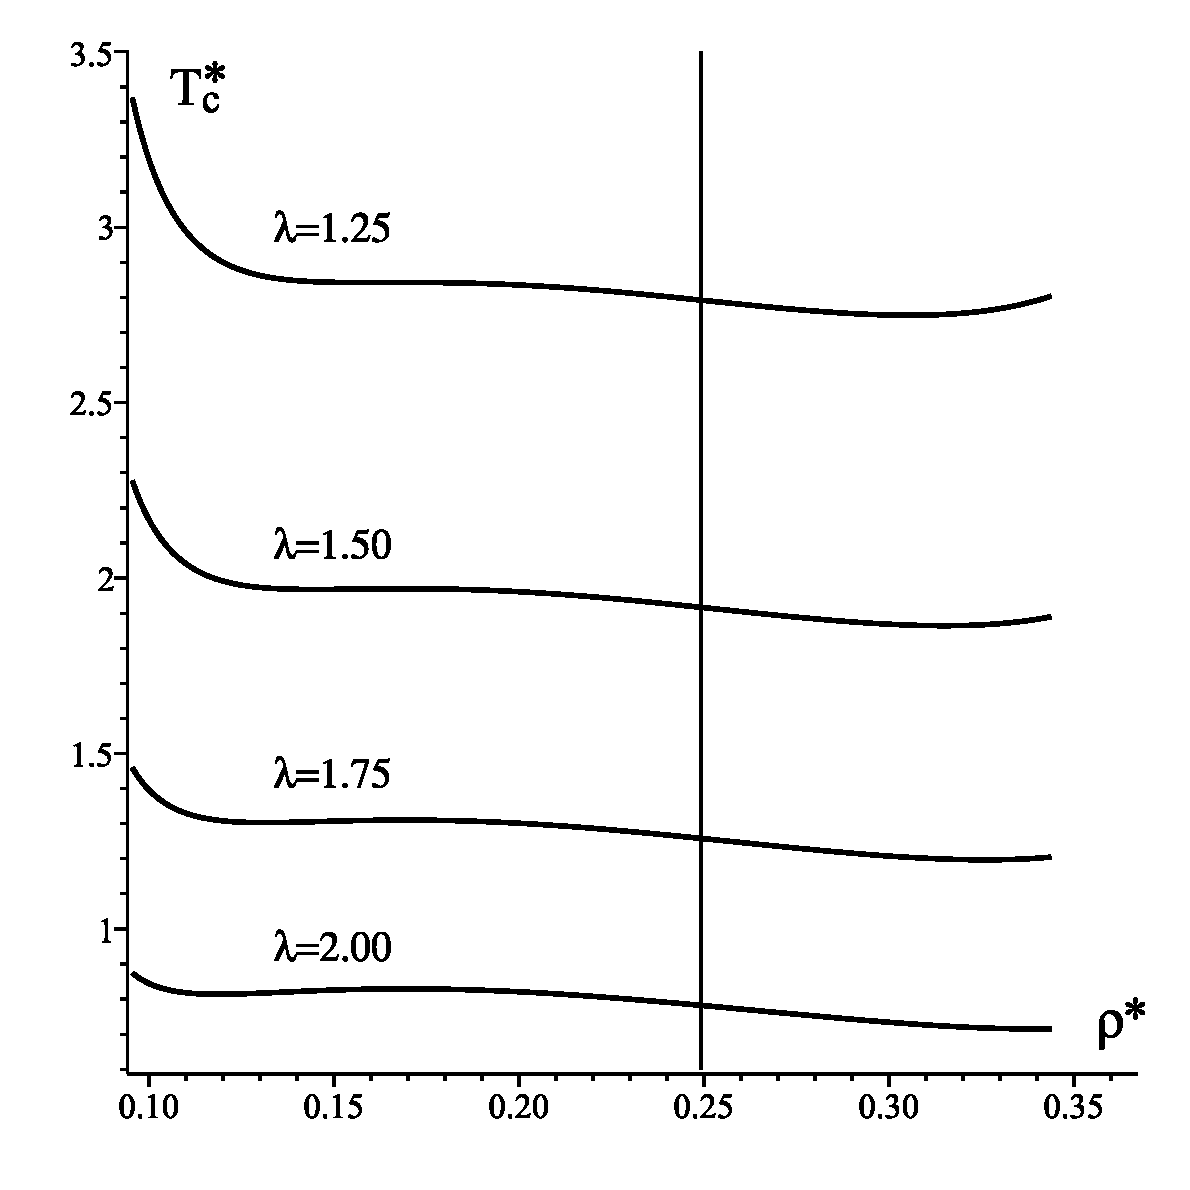
\includegraphics[width=0.45\textwidth,angle=0]{critical_temp_vs_rho}
	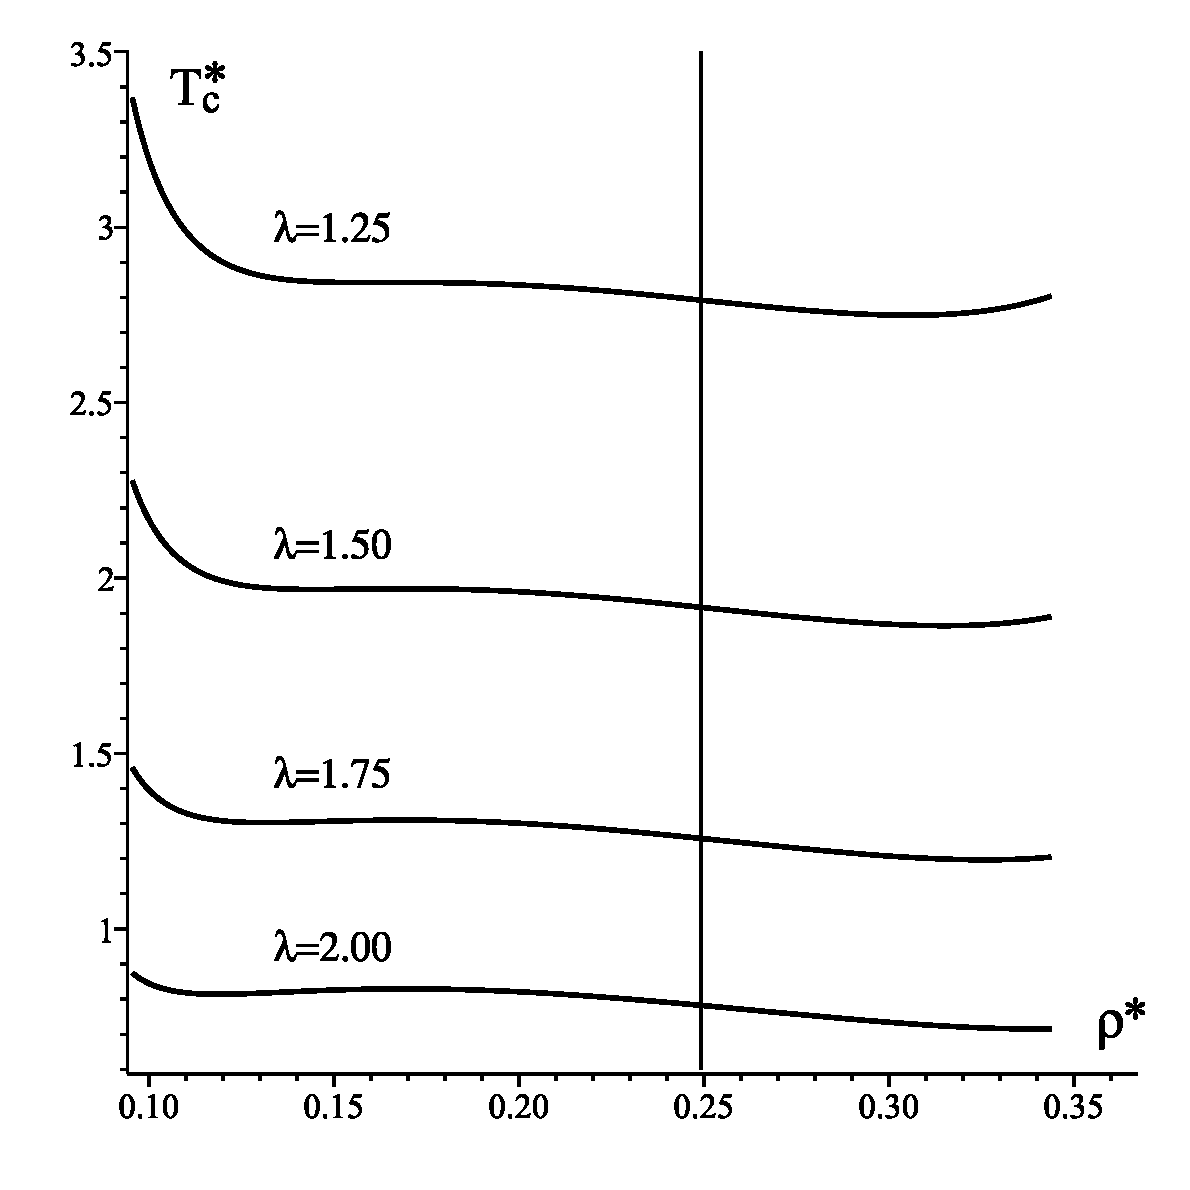
\includegraphics[width=\column]{critical_temp_vs_rho}
	\caption{Critical temperature from Eq.~\eqref{eq:T_c} versus reduced density $\rho^*$. As an example, the square-well potential is used with different values of parameter $\lambda$ (for details, see Section~\ref{sec:results}). The vertical line corresponds to the critical density $\rho^*_c=0.249$ from~\cite{YukhJSP1995}. Intersection of this line with a line $T_c^* = T_c^*(\rho^*)$ determines the critical temperature for particular potential.}
	\label{fig:t_c_vs_rho}
\end{figure}

In Section~\ref{sec:results} we calculate numerical values for $T^*_c$ following from Eq~\eqref{eq:T_c} for a few model systems of type ``hard spheres with long-range attractive tail'', and compare the results obtained from our analytical approach with known results from other works. For the hard sphere system, we employ the Carnahan-Starling approximation~\cite{CarnahanStarling1969} to calculate quantities $a_2$ and $a_4$, which enter the equation~\eqref{eq:T_c} and are explicitly given in Appendix~\ref{sec:app-a}. But first let us discuss the details of interaction potentials and applied approximations for them.


\section{\label{sec:parab_pot} Interaction potentials. Parabolic approximation}
The potential energy of the inter-particle interaction is written in the form
\begin{eqnarray*}
	U_N(\vb r^N) &=& \frac12 \underset{i\neq j}{\sum_{i=1}^N \sum_{j=1}^N} \Psi(r_{ij}) 
	+ \frac12 \underset{i\neq j}{\sum_{i=1}^N \sum_{j=1}^N} \Phi(r_{ij}).	
\end{eqnarray*}
Here $\Psi(r)$ corresponds for the short-range repulsive interaction, and $\Phi(r)$ for the long-range attractive interaction. In this work the HC potential is taken for $\Psi(r)$
\begin{equation*}
	\Psi(r) = 
	\left\{
	\begin{array}{cc}
		\infty, \quad r\leq \sigma, \\
		0, \quad r > \sigma
	\end{array}
	\right.
\end{equation*}
where $\sigma$ denotes the HC diameter. The long-range term $\Phi(r)$ is chosen so that it possesses a potential well at $r \geq \sigma$
\begin{equation}
	\label{def:long-range-potential}
	\Phi(r) = \left\{
	\begin{array}{cc}
		0, & r \leq \sigma, 
		\\
		\phi(r), & r > \sigma.
	\end{array}
	\right.
\end{equation}
where $\phi(r)$ denotes an attractive part of the interaction and is chosen in the form a few widely used potentials later.
Separation in~\eqref{def:long-range-potential} is not the only way to select the form for $\Phi(r)$ inside the HC region. One popular approach is the Weeks-Chandler-Andersen (WCA) regularization originated from~\cite{WCA1971}, according to which one has
\begin{equation}
	\label{def:long-range-potential_wca}
	\Phi(r) = \left\{
	\begin{array}{cc}
		-\varepsilon, & r \leq r_{\rm m}, 
		\\
		\phi(r), & r > \sigma.
	\end{array}
	\right.
\end{equation}
where $r_{\rm m}$ is the coordinate of the potential minimum. We use the WCA regularization schema for most of the potentials considered in Section~\ref{sec:results}.

It is additionally assumed that the attractive part of the interaction potential possesses a well behaved Fourier component $\hat{\Phi}_{\vb k}$ such that:
\begin{equation*}
	\Phi(r) = \frac{1}{V} \sum_{\vb k} \hat{\Phi}_{\vb k} {\rm e}^{i\vb k \vb r} = \frac{1}{(2\pi)^3} \int \hat{\Phi}_{\vb k} {\rm e}^{i\vb k \vb r} {\rm d} {\vb k},
\end{equation*}
and
\begin{equation*}
	\label{def:fourier}
	\hat{\Phi}_{\vb k} = \int \Phi(r) {\rm e}^{-i\vb k \vb r} {\rm d} {\vb r}.
\end{equation*}
Converting to spherical coordinates, and integrating over the angle variables, one arrives at
\begin{equation}
	\label{def:fourier_spherical}
	\hat{\Phi}(k) = \frac{4\pi}{k} \int_{0}^{\infty} r \Phi(r) \sin(k r) {\rm d} r.
\end{equation}

Several model potentials will be considered for $\phi$ in the next Section~\ref{sec:results}. 

To proceed with analytic calculations of the critical temperature and in order ot get some numerical results, let us apply the so-called parabolic approximation for the Fourier component of the interaction potential
\begin{equation*}
	\hat{\Phi}_{\vb k} = \hat{\Phi}_0 (1 - 2b^2k^2),
\end{equation*}
where 
\begin{equation*}
	2b^2 = -\frac{1}{2\hat{\Phi}_0} \frac{\partial^2 \hat{\Phi}_k}{\partial k^2} \bigg|_{k=0}.
\end{equation*}
Then let us select the cut-off parameter as
\begin{equation*}
B_0 = \frac{1}{\sqrt{2} b}.
\end{equation*}
For $\hat{\Phi}_{B_{n+1}, B_n}$, in the case of arithmetic average, it follows
\begin{equation*}
	\hat{\Phi}_{B_{n+1}, B_n} = \hat{\Phi}_0 \left(1 - s^{-2n} \frac{1 + s^{-2}}{2}\right)
\end{equation*}
and for $q$ one obtains
\begin{equation*}
	q = -\frac{\beta \hat{\Phi}_0}{V} \bar{q}, \quad \bar{q} = \frac{1 + s^{-2}}{2},
\end{equation*}
with $\bar{q} = 0.5389$.

In the case of spherical averaging
\begin{eqnarray}
	\label{def:spheric_average}
	\hat{\Phi}_{B_{n+1}, B_n} & = &  \frac{\int_{B_{n+1}}^{B_n} \hat{\Phi}_{\vb k} {\rm d} {\vb k}}
	{\int_{B_{n+1}}^{B_n} {\rm d} {\vb k}} 
	\nonumber
	\\
	& = & \frac{\hat{\Phi}_0 \int_{B_{n+1}}^{B_n} (1 - 2b^2k^2) k^2 {\rm d} k}{\int_{B_{n+1}}^{B_n} k^2 {\rm d} k}
\end{eqnarray}
one gets
\begin{equation*}
	\hat{\Phi}_{B_{n+1}, B_n} = \hat{\Phi}_0 \left(1 - s^{-2n} \frac{3(1 - s^{-5})}{5(1 - s^{-3})}\right)
\end{equation*}
and for $q$
\begin{equation*}
	q = -\frac{\beta \hat{\Phi}_0}{V} \bar{q}, \quad \bar{q} = \frac{3(1 - s^{-5})}{5(1 - s^{-3})},
\end{equation*}
with $\bar{q} = 0.6123$ at $s = s^*$.

For convenience, we gathered the numerical values of coefficients depending on the potential averaging details in Table~\ref{tab:num_coef_vs_average}.
\\

\begin{table}[h]
	\noindent\caption{Numerical values for non-universal coefficients calculated at $x^* = 0$. These are dependent on the details of potential averaging during the layer-by-layer integration.}\vskip3mm\tabcolsep4.5pt
	\begin{tabular}{|c|c|c|c|}
		\hline
		Averaging & $\bar{q}$ \quad & $\bar{r}$ & $\bar{u}$ \\
		\hline
		Arithmetic & 0.5389  & 0.5389 & 0.6890 \\
		Spherical & 0.6123 & 0.6123 & 0.8894 \\
		\hline
	\end{tabular}
	\label{tab:num_coef_vs_average}
\end{table}


\section{\label{sec:results}Results. Critical temperature for model interaction potentials}

\begin{table}[h]
	\caption{Critical temperature for different values of $R_0/\alpha$.}
	\begin{center}
		\begin{tabular}{|c|c|}
			\hline
			\multicolumn{2}{|c|}{HC Morse} \\
			\hline
			$R_0/\alpha$ \quad & $T_c^*$ \\
			\hline
			2.0  & 4.2852 \\
			2.5  & 2.1593 \\
			3.0  & 1.3418 \\
			3.5  & 0.9396 \\
			4.0  & 0.7096 \\
			4.5  & 0.5641 \\
			5.0  & 0.4652 \\
			\hline
		\end{tabular}
	\end{center}
	\label{tab:morse_temp_cr}
\end{table}

In this section we present numerical results for critical temperature calculated by Eq.~\eqref{eq:T_c} for a few van der Waals hard-core models~\cite{KreiciNezbeda2012}. We consider the following potentials as the long-range attractive part of the whole interaction: the Morse potential, the square-well potential, the Yukawa potential, and the Lennard-Jones 6-12 potential. For potential averaging we apply the spherical one~\eqref{def:spheric_average}.
%The expressions for all these potentials as well as for the corresponding Fourier transforms $\hat{\Phi}_{\vb k}$ are presented in Appendix~\ref{app:potentials}.

We start with the Morse potential given by
\begin{equation}
	%\label{def:morse}
	\phi^M(r) = \varepsilon \{\exp{[-2(r-R_0)/\alpha]}-2\exp{[-(r-R_0)/\alpha]}\}.
\end{equation}
This potential is characterized by the ratio of its parameters $R_0/\alpha$. With increasing $R_0/\alpha$, the range of interaction decreases, or in other words, the potential well becomes narrower.
Its Fourier transform is
\begin{equation*}
	\hat{\phi}^M_{\vb k} = -16\pi\varepsilon\alpha^3 {\rm e}^{R_0/\alpha} 
	\left[\frac{1}{(1 + \alpha k^2)^2} - \frac{{\rm e}^{R_0/\alpha}}{(4 + \alpha^2 k^2)^2}\right],
\end{equation*}
and the Fourier transform $\hat{\Phi}_{\vb k}$ is
\begin{eqnarray*}
	\label{eq:part_morse_fourier}
	\hat{\Phi}_k &=& -16\pi \varepsilon \alpha^3 
	\left[
	\frac{1}{1+k^2\alpha^2}\left(\frac{\sigma}{\alpha} + \frac{2}{1+k^2\alpha^2}\right) \cos(k\sigma)
	\right.
	\nonumber\\
	&& \left.
	-\frac{1}{4 + k^2\alpha^2} \left(\frac{\sigma}{\alpha} + \frac{4}{4 + k^2\alpha^2}\right) \cos(k\sigma)
	\right.
	\nonumber \\
	&& \left.
	+ \frac{\sigma/\alpha}{1 + k^2\alpha^2} \left(\frac{\sigma}{\alpha} + \frac{1 - k^2\alpha^2}{1 + k^2 \alpha^2}\right) \frac{\sin(k\sigma)}{k\sigma}
	\right.
	\nonumber\\
	&& \left.
	- \frac{\sigma/\alpha}{4 + k^2\alpha^2} \left(2\frac{\sigma}{\alpha} + \frac{4 - k^2\alpha^2}{4 + k^2\alpha^2}\right) \frac{\sin(k\sigma)}{k\sigma}
	\right].
\end{eqnarray*}
The results for critical temperature for the hard-core Morse model are presented in Table~\ref{tab:morse_temp_cr}. It is seen from the results that the critical temperature decreases as the range of interaction decreases. This trend is a common fact~\cite{KreiciNezbeda2012,MendoubWaxJakse2010}.
We have not found other works that study the hard-core Morse fluid, but we include these results here since it has been the model often considered in the collective variables approach with HS as a reference system~\cite{Yukh1990,YukhJSP1995,PatsJSP1995}, as well as without employing additional RS~\cite{PylMpkDobUPJ2023b,PylJML2023}.

\begin{table}[h]
	\caption{Critical temperature of the hard-core square-well fluid for different values of $\lambda$.}
	\begin{center}
		\begin{tabular}{|c|c|c|}
			%\begin{tabular}{cccccccccc}
			\hline
			\multicolumn{3}{|c|}{Square-well}\\
			\hline
			$\lambda$ & $T_c^*$ (WCA) & $T_c^*$ \cite{KreiciNezbeda2012} \\
			\hline
			1.25 & 0.78 & 0.75 \\
			1.50 & 1.26 & 1.25 \\
			1.75 & 1.92 & 1.88 \\
			2.00  & 2.79 & 2.72 \\
			\hline
		\end{tabular}
	\end{center}
	\label{tab:sw_temp_cr}
\end{table}

We proceed with the square-well potential given by
\begin{equation}
	\label{def:sw}
	\begin{array}{llll}
		\phi^{SW}(r) & = & \infty, & \text{if } r\leq \sigma,
		\\
		& = & -\varepsilon, & \text{if } \sigma < r \leq \lambda\sigma,
		\\
		& = & 0, & \text{if } r > \sigma.
	\end{array}
\end{equation}
This potential is characterized by the parameter $\lambda$. Increasing $\lambda$ one increases the width of the square well, and thus the range of interaction increases.
Its Fourier transform does not exist, and the Fourier transform $\hat{\Phi}_{\vb k}$ in this case is
\begin{eqnarray*}
	\hat{\Phi}_k & = & -\frac{4\pi\varepsilon\sigma^3}{(\sigma k)^3} 
	\left[\sin(\lambda \sigma k) - \lambda \sigma k \cos(\lambda \sigma k) - \sin(\sigma k) + \sigma k \cos(\sigma k)\right].
\end{eqnarray*}
We however will apply the WCA regularization for the square-well potential
in the hard-core region
\begin{equation}
	\label{def:sw-wca}
	\Phi(r) = \left\{
	\begin{array}{cc}
		-\varepsilon, & r \leq \sigma, 
		\\
		\phi^{SW}(r), & r > \sigma,
	\end{array}
	\right.
\end{equation}
since for such choice the agreement of critical temperature values with known results for this model is much better. The Fourier transform $\hat{\Phi}_{\vb k}$ in this case is
\begin{eqnarray*}
	\hat{\Phi}_k & = & -\frac{4\pi\varepsilon\sigma^3}{(\sigma k)^3} 
	\left[\sin(\lambda \sigma k) - \lambda \sigma k \cos(\lambda \sigma k)\right].
\end{eqnarray*}
The results for such model are presented in Table~\ref{tab:sw_temp_cr}. The results are compared with the ones reported in~\cite{KreiciNezbeda2012} for their perturbed virial expansion of the second order (PVE2). The work~\cite{KreiciNezbeda2012} contains more results for the hard-core square-well model obtained by different methods as well as references to computer simulation results.  
As is seen from the results, the critical temperature increases as the range of interaction increases. Overall, the agreement of the critical temperature for the square-well potential obtained within our approach agrees very well with the known results for this model.

\begin{table}[h]
	\caption{Critical temperature of the hard-core Yukawa fluid for different values of $\lambda$.}
	\begin{center}
		\begin{tabular}{|c|c|c|c|}
			%\begin{tabular}{cccccccccc}
			\hline
			\multicolumn{4}{|c|}{HC Yukawa}\\
			\hline
			$\lambda$ & $T_c^*$ & $T_c^*$ (WCA)& $T_c^*$ \cite{MendoubWaxJakse2010} \\
			\hline
			0.5 & 6.15 & 7.24 & 7.009 \\
			1.0 & 2.07 & 2.69 & 2.486 \\
			1.5 & 1.16 & 1.69 & 1.634 \\
			1.8 & 0.90 & 1.41 & 1.228 \\
			2.0 & 0.79 & 1.28 & 1.031 \\
			2.5 & 0.59 & 1.07 & 0.836 \\
			3.0 & 0.47 & 0.94 & 0.722 \\
			\hline
		\end{tabular}
	\end{center}
	\label{tab:yukawa_temp_cr}
\end{table}

The next one is the Yukawa potential give by 
\begin{equation}
	\label{def:yukawa}
	\phi^Y(r) = -\frac{\varepsilon \sigma}{r} \exp[-\lambda(r/\sigma - 1)].
\end{equation}
It is characterized by the parameter $\lambda$. With increasing $\lambda$ the potential well gets narrower, thus the range of interaction decreases.
Its Fourier transform is
\begin{equation*}
	\hat{\phi}^Y_{\vb k} = -\frac{4\pi \varepsilon \sigma^3 {\rm e}^{\lambda}}{\lambda^2 + \sigma^2 k^2},
\end{equation*}
and the Fourier transform $\hat{\Phi}_{\vb k}$ is
\begin{eqnarray*}
	\label{eq:part_yukawa_fourier}
	\hat{\Phi}_k & = & -\frac{4\pi \varepsilon\sigma^3}{(\lambda^2 + \sigma^2 k^2)}
	\left[\cos(\sigma k) + \lambda \frac{\sin(\sigma k)}{\sigma k} \right].
\end{eqnarray*}
Applying the WCA regularization, one gets
\begin{equation}
	\label{def:yukawa_wca}
	\phi^Y(r) = \left\{
	\begin{array}{ll}
		-\varepsilon, & r \leq \sigma 
		\\
		-\frac{\varepsilon \sigma}{r} \exp[-\lambda(r/\sigma - 1)], & r > \sigma,
	\end{array}
	\right.
\end{equation}
and thus
\begin{eqnarray*}
	\label{eq:wca_yukawa_fourier}
	\hat{\Phi}_k & = & -4\pi \varepsilon\sigma^3 \left\{ 
	\frac{\sin(\sigma k) - \sigma k \cos(\sigma k)}{(\sigma k)^3}
	+\frac{1}{(\lambda^2 + \sigma^2 k^2)}
	\left[\cos(\sigma k) + \lambda \frac{\sin(\sigma k)}{\sigma k} \right]
	\right\}.
\end{eqnarray*}
The results for the critical temperatures of the hard-core attractive Yukawa model~\eqref{def:yukawa} are presented in Table~\ref{tab:yukawa_temp_cr}. They are compared with the ones reported in~\cite{MendoubWaxJakse2010} (wherein other results for the critical temperature of the hard-core Yukawa model can also be found). As is seen from the Table~\ref{tab:yukawa_temp_cr}, the critical temperature decreases as the range of interaction decreases. Our results are reported for two cases, with and without applying the WCA regularization. It is seen that the critical temperature calculated without applying WCA regularization tends to be lower compared to the known results, while the one with applying it tends to be higher.

\begin{table}[h]
	\caption{Critical temperature of the hard-core Lennard-Jones fluid}
	\begin{center}
		\begin{tabular}{|c|c|}
			%\begin{tabular}{cccccccccc}
			\hline
			\multicolumn{2}{|c|}{HC Lennard-Jones}\\
			\hline
			$T_c^*$ (WCA) & $T_c^*$ \cite{SowersStanley1991} \\
			\hline
			1.43 & 1.375 \\
			\hline
		\end{tabular}
	\end{center}
	\label{tab:lj_temp_cr}
\end{table}

The final potential we consider in this paper is the Lennard-Jones one
\begin{equation}
	\phi^{LJ}(r) = 4\varepsilon \left[(\sigma/r)^{12} - (\sigma/r)^6\right].
\end{equation}
The hard-core Lennard-Jones fluid is defined in literature~\cite{SowersStanley1991,DiezLargoSolana2010} as
\begin{equation}
	\phi^{LJ}(r) = \left\{
	\begin{array}{llll}
		\infty, & r\leq \sigma,
		\\
		-\varepsilon, & \sigma < r \leq r_{\rm m}, 
		\\
		4\varepsilon \left[(\sigma/r)^{12} - (\sigma/r)^6\right], & r > r_{\rm m},
	\end{array}
	\right.
\end{equation}
where $r_{\rm m}=2^{1/6}\sigma$.
In this case it is easy to apply the WCA regularization
\begin{equation}
	\label{def:lj_wca}
	\Phi(r) = \left\{
	\begin{array}{ll}
		-\varepsilon, & r \leq r_{\rm m},
		\\
		4\varepsilon \left[(\sigma/r)^{12} - (\sigma/r)^6\right], & r > r_{\rm m}.
	\end{array}	
	\right.
\end{equation}
We do not present the explicit formula for the Fourier transform of potential defined by~\eqref{def:lj_wca}, since it is somewhat cumbersome, but its calculation by~\eqref{def:fourier_spherical} is straightforward. 
The calculated critical temperature is present in Table~\ref{tab:lj_temp_cr}. Result from~\cite{SowersStanley1991} is given for comparison.



\section{Conclusions}
Having integrated the functional for the grand partition function of a system of many interacting particles applying the ``layer-by-layer'' approach, we obtained a sequence of effective block Hamiltonians each characterized by its own coefficients. Since the approach is in essence an analytical one, and the coefficients are known explicitly, the recurrence relations were written down. The analysis of the recurrence relations showed the existence of a fixed-point solution. The coordinates of the fixed point were found, as well as a solution linearized near the fixed point was presented. From the condition that at large iteration number $n$ the linearized solution must be equal to the fixed-point solution, we found explicit equation for the critical temperature $T^*_c$ as a function of particle density $\rho^*$. Taking the value for the critical density from another work~\cite{YukhJSP1995}, we found the critical temperature that depends only on the parameters of the attractive part of the interaction potential. Based on this equation, the critical temperature was calculated for several hard-core van der Waals fluids and compared with known results for the considered models. The results confirm that the critical temperature of simple fluid models decreases as the range of attractive interaction decreases.

\appendix

\renewcommand{\theequation}{A.\arabic{equation}}
\setcounter{equation}{0}

\section{\label{sec:app-a} Explicit expressions for quantities entering the GPF functional}
Here we explicitly present quantities entering the GPF expressions~\eqref{Xi_L} and~\eqref{Xi_L_1}.
%\begin{equation}
%	\label{tilde_frak_M0}
%	\tilde{\frak M}_0 = \frak M_0 + (h + {\frak M_3}/{\frak M_4})\tilde{\frak M}_1 - \frac{\alpha(0)}{2}\tilde{\frak M}_1^2,
%\end{equation}

First, for the coefficients in~\eqref{Xi_L} one has
\begin{eqnarray*}
	\label{tilde_frak_M0}
	\tilde{\mathfrak M}_0 & = & \langle N \rangle_0 
	\left[
		\tilde{\mathfrak{m}}_0
		+ \left(h + \frac{\mathfrak{m}_3}{\mathfrak{m}_4} \right) \tilde{\mathfrak{m}}_1
		- \frac{\beta \hat{\Phi}_0}{2}\frac{\langle N \rangle_0}{V} \tilde{\mathfrak{m}}_1^2.
	\right],
\\
	\tilde{\mathfrak{m}}_0 & = & -\frac{\mathfrak{m}_1 \mathfrak{m}_3}{\mathfrak{m}_4} + \frac{\mathfrak{m}_2 \mathfrak{m}^2_3}{2 \mathfrak{m}_4^2} - \frac{\mathfrak{m}_3^4}{8\mathfrak{m}_4^2},
\\
	\tilde{\mathfrak{m}}_1 & = & \mathfrak{m}_1 - \frac{\mathfrak{m}_2 \mathfrak{m}_3}{\mathfrak{m}_4} + \frac{\mathfrak{m}_3^3}{3\mathfrak{m}_4^2},
\end{eqnarray*}
where $\langle N \rangle_0$ is the average particle number for the RS, and
\begin{eqnarray*}
	\mathfrak{m}_1 & = & 1,
	\\
	\mathfrak{m}_2 & = & 1 + \rho \hat{h}^{(2)},
	\\
	\mathfrak{m}_3 & = & 1 + 3\rho \hat{h}^{(2)} + \rho^2 \hat{h}^{(3)},
	\\
	\mathfrak{m}_4 & = & 1 + 7\rho \hat{h}^{(2)} + 6\rho^2 \hat{h}^{(3)} + \rho^3 \hat{h}^{(4)}.
\end{eqnarray*}
Here $\hat{h}^{(n)}$ are the Fourier transforms of the total correlation functions at $\abs{\vb k} = 0,$ and $\mathfrak{m}_n$ are the $n$-particle structure factors at $\abs{\vb k} = 0$, both determined for the RS. They are functions of the RS particle density. More detailed investigation of quantities $\mathfrak{m}_n$ and $\hat{h}^{(n)}$ was performed in~\cite{RomaJPS2024,Roma2023Preprint}.

The quantity $h$ stands for
\begin{equation*}
	h = \beta(\mu - \mu_0),
\end{equation*}
where $\mu$ and $\mu_0$ are the chemical potentials of the whole system and of the RS, respectively.

The quantity $Q(\tilde{\mathfrak{M}}_2, \mathfrak{M}_4)$ is determined by
\begin{equation*}
	\label{quantity_Q}
	Q(\tilde{\mathfrak{M}}_2, \mathfrak{M}_4) = \frac{1}{2\sqrt{\pi}} \left(\frac{12}{N_0 \langle N \rangle_0\abs{\mathfrak{m}_4}}\right)^{1/4} {\rm e}^{y^2/2} U(0,y)
\end{equation*}
where
\begin{eqnarray*}
	y & = & \left(\frac{\langle N \rangle_0}{N_0} \frac{3\tilde{\mathfrak{m}}_2^2}{\abs{\mathfrak{m}_4}}\right)^{1/2},
	\\
	\tilde{\mathfrak{m}}_2 & = & \mathfrak{m}_2 - \frac{\mathfrak{m}_3^2}{2\mathfrak{m}_4},
\end{eqnarray*}
and $U(a, y)$ is the Weber parabolic cylinder function~\cite{nistMathFuncHandbook2010}.

Now, for quantities in~\eqref{Xi_L_1} one has
\begin{eqnarray*}
	a_2 & = & \left(\frac{3}{N_0 \langle N \rangle_0 \abs{\mathfrak{m}_4}}\right)^{1/2} U(y),
	\\
	a_4 & = & \frac{3}{N_0 \langle N \rangle_0 \abs{\mathfrak{m}_4}} \varphi(y),
\end{eqnarray*}
where
\begin{eqnarray*}
	U(y) & = & \frac{U(1,y)}{U(0,y)},
	\\
	\varphi(y) & = & 3U^2(y) + 2yU(y) -2.
\end{eqnarray*}
By multiplying $a_2$ by $\langle N \rangle_0$, and $a_4$ by $\langle N \rangle_0^2$, we get quantities that are functions of the particle density only
\begin{eqnarray*}
	a_2^{'} & = & \langle N \rangle_0 a_2,
	\\
	a_4^{'} & = & \langle N \rangle_0^2 a_4.
\end{eqnarray*}

Finally, the quantity $\mu^*$ is a linear function of the chemical potential $\mu$
\begin{equation*}
	\mu^* = h + \frac{\mathfrak{m}_3}{\mathfrak{m}_4} + \frac{\langle N \rangle_0}{V} \beta\hat{\Phi}_0 \tilde{\mathfrak{m}}_1.
\end{equation*}

\section{\label{sec:app-b} Some relations for site variables}

Here we present some relations between sets of CV $\{\rho_{\vb k}, \omega_{\vb k}\}$ and their counterparts -- site CV $\{\tilde{\rho}_{\vb l}, \tilde{\omega}_{\vb l}\}$. The presented expressions are meant to be generic, so that the meaning of summation over $\vb k$ and over $\vb l$ are not particularly specified, while $N$ being the number of different values that $\vb k$ or $\vb l$ takes on. They are usually specified more strictly in particular applications.

By definition
\begin{eqnarray*}
	\tilde{\omega}_{\vb l} & = & \frac{1}{\sqrt{N}} \sum_{\vb k} \omega_{\vb k} {\rm e}^{-{\rm i}{\vb k}{\vb l}},
\\
	\tilde{\rho}_{\vb l} & = & \frac{1}{\sqrt{N}} \sum_{\vb k} \rho_{\vb k} {\rm e}^{{\rm i} {\vb k} {\vb l}}.
\end{eqnarray*}

From this definition the following equalities follow.
\begin{eqnarray*}
	\sum_{\vb l} \tilde{\omega}_{\vb l} \tilde{\rho}_{\vb l} & = & \sum_{\vb k} \omega_{\vb k} \rho_{\vb k}.
\end{eqnarray*}
\begin{eqnarray*}
	\sum_{\vb l} \tilde{\omega}_{\vb l}^2 & = & \sum_{\vb k} \omega_{\vb k} \omega_{-\vb k},
\\
	N \sum_{\vb l} \tilde{\omega}_{\vb l}^4 & = & \sum_{\vb k_1, \dotsc, \vb k_4} \omega_{\vb k_1} \dotsc \omega_{\vb k_4} \delta_{\vb{k}_1 + \dotsc + \vb{k}_4},
\\
	N^{\frac{n}{2} - 1} \sum_{\vb l} \tilde{\omega}_{\vb l}^n & = &  \sum_{\vb k_1, \dotsc, \vb k_n} \omega_{\vb k_1} \dotsc \omega_{\vb k_n} \delta_{\vb{k}_1 + \dotsc + \vb{k}_n}.
\end{eqnarray*}
\begin{eqnarray*}
	\sum_{\vb l} \tilde{\rho}_{\vb l}^2 & = & \sum_{\vb k} \rho_{\vb k} \rho_{-\vb k},
\\
	N \sum_{\vb l} \tilde{\rho}_{\vb l}^4 & = & \sum_{\vb k_1, \dotsc, \vb k_4} \rho_{\vb k_1} \dotsc \rho_{\vb k_4} \delta_{\vb{k}_1 + \dotsc + \vb{k}_4},
\\
	N^{\frac{n}{2} - 1} \sum_{\vb l} \tilde{\rho}_{\vb l}^n & = & \sum_{\vb k_1, \dotsc, \vb k_n} \rho_{\vb k_1} \dotsc \rho_{\vb k_n} \delta_{\vb{k}_1 + \dotsc + \vb{k}_n}.
\end{eqnarray*}

\vskip3mm \textit{}

%\bibliography{fluids_cv,fluids_general,icmp,books_cv,romanik,books_romanik_bibliography}
\bibliography{extracted}

\vspace*{-5mm} \rezume{%
Р.В. Романік, І.Р. Юхновський} {Визначення критичної температури флюїдів. Аналітичний підхід на основі методу колективних змінних} {Проведено поетапне інтегрування функціоналу великої статистичної суми системи багатьох взаємодіючих частинок}{\textit{К\,л\,ю\,ч\,о\,в\,і\,
с\,л\,о\,в\,а:} прості плини, колективні змінні, критична температура.}
\end{document}
